\documentclass{beamer}
\usepackage[utf8]{inputenc}
%\usepackage{minted}
\usepackage{amsmath}
\usepackage{fancyvrb}
\usepackage{xspace}
\usepackage{listings}
\usepackage[3D]{movie15}
\usefonttheme{structurebold}
\mode<presentation>
{
  \usetheme{default}
   \setbeamercolor{structure}{fg=black!70}
  \setbeamercovered{invisible}
  \setbeamerfont{title}{size=\large}
}
\usepackage[english]{babel}
\usepackage{times}
\usepackage[T1]{fontenc}
\usepackage{algorithmic}
%\usepackage[unicode]{hyperref}%$AA 3:55, 720AM 3:40, $748.80 OZAOZF
%how our code can be useful to ERDC in the future
%labwide resource on numerics; and solving problems related to numerical methods and new physical formulations (e.g. femlab)
%maybe add a couple of simulations
\hypersetup{unicode=true,colorlinks=true,linkcolor=white,urlcolor=blue}

%% The Proteus toolkit evolved to support research on new models for
%% coastal and hydraulic processes and improvements in numerical
%% methods. The models considered include multiphase flow in porous
%% media, shallow water flow, turbulent free surface flow, and
%% flow-driven processes such as sediment and species transport. Python
%% was used for implementing high-level class hierarchies and prototyping
%% new algorithms, while performance critical sections were optimized
%% using compiled languages. We discuss the toolkit design,
%% performance, and open issues.

\newcommand{\email}[1]{\href{mailto:#1}{\texttt{#1}}}
%differential operators
\newcommand{\grad}{\nabla}
\newcommand{\deld}{\nabla \cdot}
\newcommand{\lap}{\Delta}
%boldface in math mode
\newcommand{\bm}[1]{\mbox{{\boldmath ${#1}$}}}
% vectors and tensors
\renewcommand{\vec}[1]{{\bf #1}}
\newcommand{\gvec}[1]{\mbox{{\boldmath ${#1}$}}}
%mwf comment out bar
%\newcommand{\ten}[1]{\bar{\bm{#1}}}
\newcommand{\ten}[1]{\bm{#1}}
%derivatives
\newcommand{\od}[2]{\frac{d {#1}}{d {#2}}}
\newcommand{\ods}[2]{\frac{d^2{#1}}{d {{#2}^2}}}
\newcommand{\pd}[2]{\frac{\partial {#1}}{\partial {#2}}}
\newcommand{\pds}[2]{\frac{\partial^2{#1}}{\partial {{#2}^2}}}
\newcommand{\pdsm}[3]{\frac{\partial^2{#1}}{\partial {#2}\,\partial {#3}}}
%funtional analysis
\newcommand{\abs}[1]{\left| #1 \right|}
\newcommand{\norm}[1]{\left\| #1 \right\|}
\newcommand{\iprod}[2]{\left( #1, #2 \right)}
\newcommand{\dprod}[2]{\left\langle #1, #2 \right\rangle}
%real numbers
\newcommand{\field}[1]{\mathbb{#1}}
\newcommand{\R}{\field{R}}
\renewcommand{\P}{\field{P}}
\newcommand{\T}{\mathcal{T}}
%funciton spaces
\newcommand{\M}{\mathcal{M}}
%delimiters
\newcommand{\pl}{\left(}
\newcommand{\pr}{\right)}
\newcommand{\sbl}{\left[}
\newcommand{\sbr}{\right]}
\newcommand{\dbl}{\left[\hspace{-0.05cm}\left[}
\newcommand{\dbr}{\right]\hspace{-0.05cm}\right]}
\newcommand{\cbl}{\left\{ }
\newcommand{\cbr}{\right\} }
\newcommand{\eqn}[1]{equation \ref {eq:#1}} 
\newcommand{\Eqn}[1]{Equation \ref {eq:#1}} 
\newcommand{\eqnst}[2]{equations \ref{eq:#1} and \ref{eq:#2}} 
\newcommand{\Eqnst}[2]{Equations \ref{eq:#1} and \ref{eq:#2}} 
\newcommand{\eqns}[2]{equations \ref{eq:#1}--\ref{eq:#2}} 
\newcommand{\Eqns}[2]{Equations \ref{eq:#1}--\ref{eq:#2}}
\newcommand{\msection}[1]{ \vspace{.2in} {\noindent \bf #1}.}
%\renewcommand{\for}{\mbox{for}\quad}
\newcommand{\for}{\mbox{for}\quad}
\newcommand{\argmin}{\mbox{argmin}}
\newcommand{\argmax}{\mbox{argmax}}
\newcommand{\fig}[1]{figure \ref{fig:#1}} 
\newcommand{\Fig}[1]{Figure \ref{fig:#1}} 
\newcommand{\figst}[2]{figures \ref {fig:#1} and \ref {fig:#2}} 
\newcommand{\Figst}[2]{Figures \ref {fig:#1} and \ref {fig:#2}} 
\newcommand{\figs}[2]{figures \ref{fig:#1}--\ref{fig:#2}} 
\newcommand{\Figs}[2]{Figures \ref{fig:#1}--\ref{fig:#2}}
\newcommand{\tab}[1]{table \ref {tab:#1}} 
\newcommand{\Tab}[1]{Table \ref {tab:#1}} 
\newcommand{\tabst}[2]{tables \ref {tab:#1} and \ref {tab:#2}} 
\newcommand{\Tabst}[2]{Tables \ref {tab:#1} and \ref {tab:#2}} 
\newcommand{\tabs}[2]{tables \ref{tab:#1}--\ref{tab:#2}} 
\newcommand{\Tabs}[2]{Tables \ref{tab:#1}--\ref{tab:#2}}
%\newtheorem{theorem}{Theorem}
\newenvironment{neqnarray}[1]{\begin{minipage}[t]{6.5in}  \begin{minipage}[b]{1.0in} #1 \end{minipage}  \begin{minipage}[b]{5.5in}\begin{eqnarray}}{\end{eqnarray}\end{minipage}\end{minipage}}
\newcommand{\bneqnarray}[2]{\\ \\ \fbox{\begin{neqnarray}{#1} #2 \end{neqnarray}}\\ \\ \noindent}

%%%mwf begin adding things
%physical quantities
\newcommand{\source}{b} %or d? or ...
\newcommand{\dx}{\, \mathrm{d}\vec x} 
\newcommand{\ds}{\, \mathrm{d}s}

%finite element quantities
%\newcommand{\Mh}{\mathcal{M}^h}
\newcommand{\Mh}{T_h}
\newcommand{\RT}{$\mbox{RT}_0$}

%\newcommand{\elem}{\mathcal{E}}
%\newcommand{\face}{e}
%\newcommand{\node}{\vec x}
%\newcommand{\nodestar}[1]{\Omega^{#1}}

%element
\newcommand{\elem}{\Omega}
%element boundary (ind. of element)
%\newcommand{\face}{\partial \Omega}
\newcommand{\face}{\gamma}
%mesh nodes
\newcommand{\node}{\vec x}
%node star
\newcommand{\nodestar}[1]{\mathcal{E}({#1})}
%faces in element not on Neumann boundary
\newcommand{\dirIntFaces}[1]{\mathcal{F}_{i}({#1})}
%nodes beloging to an element
\newcommand{\elemnodes}[1]{\mathcal{N}({#1})}
%nodes beloging to an element boundary
\newcommand{\facenodes}[1]{\mathcal{N}({#1})}
%left and right elements at a face
\newcommand{\lelem}{\Omega_{\ell}}
\newcommand{\relem}{\Omega_{r}}
%the left and right identifiers
\newcommand{\eleft}[1]{e_{\ell}({#1})}
\newcommand{\eright}[1]{e_{r}({#1})}
%local numbering on nodestars
\newcommand{\elemstar}{e^{\ast}}
\newcommand{\estarleft}[1]{e^{\ast}_{\ell}({#1})}
\newcommand{\estarright}[1]{e^{\ast}_{r}({#1})}
%left and right normals to face
\newcommand{\lnormal}{\vec{n}_{\ell}}
\newcommand{\rnormal}{\vec{n}_{r}}
%unique normal on face
\newcommand{\fnormal}{\vec{n}_{f}}
%local indeces on left and right
\newcommand{\ileft}{i_{\ell}}
\newcommand{\iright}{i_{r}}
%jump operator
%mwf orig
%\newcommand{\jump}[1]{\dbl #1 \dbr}
%\newcommand{\jump}[2][-0.075cm]{\left[\hspace{#1} \left[ #2 \right]\hspace{#1} \right]}
\newcommand{\jump}[2][\!]{\left[ #1 \left[ #2 \right]#1 \right]}
%multiscale formalism
\newcommand{\strongRes}{\mathcal{R}}
\newcommand{\Lop}{\mathcal{L}}
\newcommand{\LopStar}{\mathcal{L}^{\ast}}
\newcommand{\Ls}{\mathcal{L}_s}
\newcommand{\LsStar}{\mathcal{L}_s^{\ast}}
\newcommand{\LsStarApprox}{\mathcal{L}^{\ast}_{s,h}}
\newcommand{\LsHat}{\hat{\mathcal{L}}_s}
%richards equation stuff
\newcommand{\psk}{$p$-$s$-$k$}

%tables and display convenience
\newcommand{\tx}[1]{$\times 10^{#1}$}
\newcommand{\bit}{\begin{itemize}}
\newcommand{\eit}{\end{itemize}}
\newcommand{\frt}[1]{\frametitle{#1}}

\title[petsc4py]{Lessons Learned and Open Issues from the Development of the Proteus Toolkit for Coastal and Hydraulics Modeling}
\subtitle[]{\href{https://adh.usace.army.mil/proteus}%
           {\texttt{https://adh.usace.army.mil/proteus}}}
%\author[C.~Kees\inst{1} \and M.~Farthing\inst{1}]%
\author[C.~Kees \and M.~Farthing]%
{
%  Chris~Kees\inst{1} \and ~~~~~Matthew~Farthing\inst{1}\\ 
  Chris~Kees \and ~~~~~Matthew~Farthing\\ 
  \email{christopher.e.kees@usace.army.mil} \and \email{matthew.w.farthing@usace.army.mil}
}
\institute[ERDC]
{
%  \inst{1}%
  Coastal and Hydraulics Laboratory\\
  US Army Engineer Research and Development Center\\
  Vicksburg, MS
}
\date [CSE '11]
{
  SIAM CSE 2011\\
  February 28 -- March 4, 2011\\
  Reno, Nevada
}
\pgfdeclareimage[height=0.5cm]{corps_logo}{corps_logo}
\logo{\pgfuseimage{corps_logo}}

%\AtBeginSection[]
%{
%  \begin{frame}
%    \tableofcontents[currentsection]
%  \end{frame}
%}

%\AtBeginSubsection[]
%{
%  \begin{frame}<beamer>
%    \frametitle{Outline}
%    \tableofcontents[currentsection,currentsubsection]
%  \end{frame}
%}

\newcommand{\Cpp}{C\protect\raisebox{.18ex}{++}\xspace}

\begin{document}

\begin{frame}
  \titlepage
\end{frame}

\begin{frame}
  \frametitle{Outline}
  \tableofcontents
\end{frame}

\section{Overview}

\begin{frame}
\frt{What is Proteus?}
\bit
\item Proteus is a Python package for rapidly developing computer models and numerical methods.
\item The package contains a collection of modules implemented in C,C++,Fortran, and Python.
\item The implementation uses standard software engineering practices:
  object-oriented programming, loose coupling, iterative/incremental
  programming, ``literate'' programming.
\item A strong boundary is maintained between physics implementation
  and numerical methods implementation (loose coupling).
\item Has a layered API for model implementation. Highly optimized
  models for specific/detailed physics can be implemented by deriving
  from more generic models (iterative programming).
\item Contains ``wrapper'' modules for a wide variety of 3rd party
  libraries (ADH, PETSc, triangle, tetgen,...)  \eit
\end{frame}

\begin{frame}
\frametitle{History of Proteus}
\begin{itemize}
\item USACE begin development on the ADaptive Hydraulics (ADH) code in
  the 90's.
\item ADH is a C library/executable implementing parallel,
  $h$-adaptive, piecewise linear finite element methods for a variety
  of single-phase flow and transport models.
\item In 2006 we started two research projects focused on continuum
  models of multi-phase flow at various scales.
\item We decided to write a prototype for a new version of ADH with
  new models and methods as part of the research on multi-phase flow.
\item Desired characteristics of the prototype: multi-level,
  multi-scale, multi-phase/component, variable-order,
  variable-continuity, highly modular, and customizable.
\end{itemize}
\end{frame}

%2
\begin{frame}
\frt{Equations Solved}
\bit
\footnotesize
\item 2D \& 3D incompressible Navier-Stokes (Unsteady/Steady, LES,
  RANS, VANS)
\item 2D diffusive wave (overland flow)
\item 2D shallow water
\item 2D \& 3D two-phase incompressible, immiscible flow (hybrid
  VOF/level set formulation with LES, etc.)
\item 2D \& 3D saturated groundwater
\item 2D \& 3D Richards' equation (variably saturated groundwater,
  various constitutive models)
\item 2D \& 3D two-phase flow in porous media (continuum mixture
  formulation, incompressible or compressible)
\item 2D \& 3D density-dependent groundwater flow and salinity
  transport
\item 2D \& 3D eikonal equation (signed distance calculations)
\item 2D \& 3D linear elasticity
\item 3D elastoplastic deformation (levee stability, Mohr-Coulomb material)
\item 2D \& 3D 6DOF solid/air/water interaction
\item 1D,2D,\& 3D Poisson, Burgers, linear/nonlinear ADRE, Stokes,
  etc.  \eit
\end{frame}

%3 
\begin{frame}
\frt{Framework}
\begin{center}
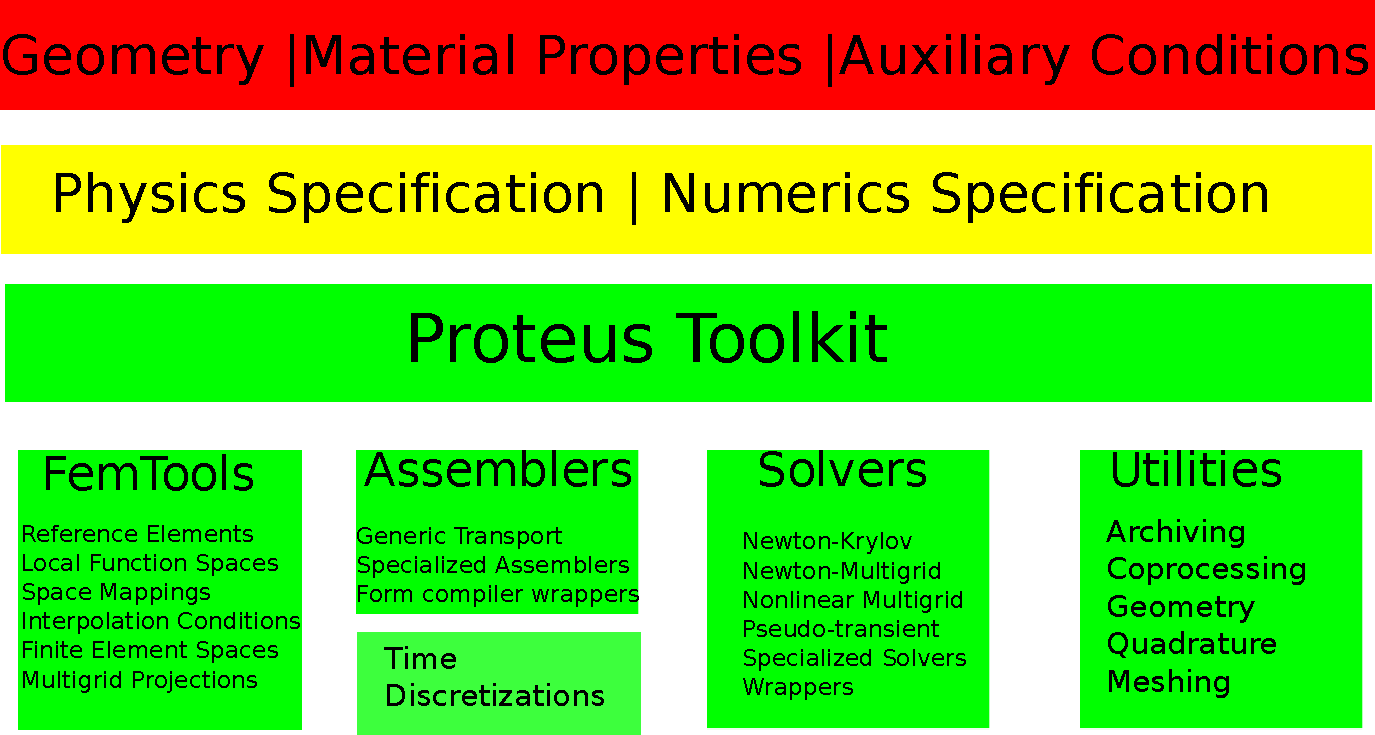
\includegraphics[scale=0.4]{modules.pdf}
\end{center}
\end{frame}


%5
\begin{frame}
\frametitle{Verified Numerics}
\bit
\footnotesize
\item Continuous linear and quadratic polynomial spaces ($C^0 P^1$ and
  $C^0 P^2$) on simplicial elements (intervals, triangles, tetrahedra)
  with nodal (Lagrange) basis
\item Continuous tensor product spaces ($C^0 Q^k$) on hexahedra with
  nodal basis
\item Discontinuous complete polynomial spaces ($C^{-1} P^k$) on
  simplicial elements with monomial basis
\item $P^1$ non-conforming simplicial elements (equivalent to
  Raviart-Thomas mixed element)
\item Eulerian-Lagrangian Localized Adjoint Methods (ELLAMs) for
  advection-dominated processes
\item Locally discontinuous Galerkin mixed elements with static
  condensation
\item SIPG/NIPG/IIPG primal discontinuous elements
\item Residual-based variational multiscale methods (RBVMS)
\item Analytical Riemann solvers (numerical fluxes) for linear
  advection, two-phase flow in porous media, and shallow water
\item Approximate Riemann solvers: Harten-Lax-van Leer (SWE), Rusanov
  (two-phase flow), Cheng-Shu (Hamilton-Jacobi)
\item Velocity post-processing to enforce element-wise (local)
  conservation \eit
\end{frame}

%6
\begin{frame}
  \frametitle{Verification and Validation Test Problems}
  \begin{minipage}{0.5\textwidth}
    \bit
  \item Dam break experiments
  \item Marin free surface flow/object experiment
  \item Wigley hull tow tank experiment
  \item Beach erosion board
  \item Flow around a cylinder
  \item Driven cavity
  \item Rotating Gaussian
  \item Advection in a vortex
  \item Porous media, slope stability,...
    %\item Poisseulle, Couette, and Decay of Vortex (low RE analytical solutions) 2D \& 3D
    \eit
  \end{minipage}\begin{minipage}{0.5\textwidth}
    \begin{overlayarea}{\textwidth}{\textwidth}
      \only<+>{\includemovie[controls,poster]{\textwidth}{\textwidth}{sloshbox2d.mov}}
      %      \only<+>{\includemovie[controls,poster]{\textwidth}{\textwidth}{dambreak2d.mov}}
      %      \only<+>{\includemovie[controls,poster]{\textwidth}{\textwidth}{sloshbox3d.mov}}
      \only<+>{\includemovie[controls,poster]{\textwidth}{\textwidth}{obstacle3d.mov}}
      %      \only<+>{\includemovie[controls,poster]{\textwidth}{\textwidth}{embankment.mov}}
    \end{overlayarea}
  \end{minipage}
\end{frame}

%7
\begin{frame}
\frt{Peer-Reviewed Verification and Validation}
\bit
\footnotesize
\item Implementation of Discontinuous Galerkin Methods for the
  Level-Set Equation on Unstructured Meshes, M. W. Farthing and C. E.
  Kees (2008) U.S. Army Engineer Research and Development Center,
  Coastal and Hydraulics Laboratory, Coastal and Hydraulics Technical
  Note, CHETN-XIII-2.

\item Locally conservative, stabilized finite element methods for
  variably saturated flow. C. E. Kees, M. W. Farthing, and C. N.
  Dawson (2008) {\em Computer Methods in Applied Mechanics and
    Engineering}, 197, 4610-4625.

\item Locally Conservative, Stabilized Finite Element Methods for a
  Class of Variable Coefficient Navier-Stokes Equations, C. E. Kees
  and M. W. Farthing (2009) ERDC-CHL TR-09-12.

\item A review of methods for moving boundary problems, C. E. Kees,
  M. W. Farthing, R. C. Berger, and T. C. Lackey (2009) ERDC-CHL
  TR-09-10.

\item Evaluating finite element methods for the level-set equation,
  M. W. Farthing and C. E. Kees (2009) ERDC-CHL TR-09-11.

\item A conservative level set method for variable-order
  approximations and unstructured meshes. C. E. Kees, I. Akkerman,
  M. W. Farthing, and Y. Bazilevs (2011) {\em Journal of Computational
    Physics}, doi:10.1016/j.jcp.2011.02.030.
\eit
\end{frame}

\section{Physics API}

\begin{frame}
\frametitle{Some Characteristics of Popular Math Software}
\begin{itemize}
\item Directed at an abstract formulation covering an important class
  of problems: $A \vec x = \vec b$, $\vec F(t,\vec y, \vec y') = 0$
\item Have multiple layers of interfaces: \texttt{dgbsv} (simple
  interface), \texttt{dgbtrf} + \texttt{dgbtrs} (computational
  interface)
\item Use robust and accurate numerics: LU with partial pivoting, BDF
  methods.
\item Some separation between problem/data description and numerics
  (PetscMat,PetscKSP).
\end{itemize}
\end{frame}

\begin{frame}
\frametitle{Popular Modeling Toolkit for PDE's}

\begin{itemize}
\item ``The COMSOL \begin{footnotesize}multiphysics simulation
  environment facilitates all steps in the modeling process: defining
  your geometry, specifying your physics, meshing, solving and then
  post-processing your results.\end{footnotesize}''

\item ``FEniCS \begin{footnotesize}is free software for automated
  solution of differential equations. We provide software tools for
  working with computational meshes, finite element variational
  formulations of PDEs, ODE solvers and linear
  algebra.\end{footnotesize}''

\item ``...OpenFOAM \begin{footnotesize}is a flexible set of efficient
  C++ modules. These are used to build a wealth of: solvers, to
  simulate specific problems in engineering mechanics; utilities, to
  perform pre- and post-processing tasks ranging from simple data
  manipulations to visualisation and mesh processing; libraries, to
  create toolboxes that are accessible to the solvers/utilities, such
  as libraries of physical models.\end{footnotesize}''
\end{itemize}
\end{frame}

\begin{frame}
\frametitle{Second Order Nonlinear, Heterogeneous Transport Systems}
Our target problems are systems of nonlinear equations governing the
transport of an abstract vector of components $u_j,j=1,\ldots,n_c$:
\begin{equation*}
\pd{m^i}{t} + \deld \pl \vec f^i - \sum_k \ten{a}^{ik} \grad \phi^k
\pr + r^i + h^i(\grad u) = 0
\end{equation*}
where $i=1,\ldots n_c$. The large majority of models in hydrology are
in this class.
\end{frame}

\begin{frame}
\frametitle{Main elements of a computer model}
\begin{itemize}
\item A set of PDE's.
\item A set of space-time domains.
\item Initial/boundary conditions and material properties.
\item Discretizations for PDE's and solvers for finite dimensional
  systems.
\item Auxiliary computations, post-processing schemes, visualization,
  archiving,...
\end{itemize}
We divide these elements into the \alert{p-file} (problem description
module), \alert{n-file} (numerics module), and \alert{batch} file.
\end{frame}

\begin{frame}
\frametitle{A simple example} For $(t,x,y) \in [0,T] \times [0,1]
\times [0,1]$ find $u$ such that
\begin{eqnarray*}
(Mu)_t + \deld \sbl \vec B u- \ten{A} \grad u \sbr&=& 0 \\ u(0,x,y)
  &=& 0 \\ u(t,x,0) &=& u(t,0,y) = 1 \\ u(t,x,1) &=& u(t,1,x) = 0
  \\ M&=&1\\ \vec{B}&=&(1,1)\\ \ten{A}&=&0.001 \ten{I}
\end{eqnarray*}
\end{frame}

\begin{frame}
\frametitle{\texttt{ladr\_2d\_p.py}} \small
\lstinputlisting{ladr_2d_p.py}
\end{frame}

\begin{frame}
\frametitle{\texttt{ladr\_2d\_c0p1\_n.py}}
\small
\lstinputlisting{ladr_2d_c0p1_n.py}
\end{frame}

\begin{frame}
\frametitle{A multi-physics example}
\small
\lstinputlisting{twp_navier_stokes_sloshbox_2d_so.py}
\end{frame}

\begin{frame}
\frametitle{\texttt{adr.py}}
\small
\lstinputlisting[lastline=12]{adr.py}
\end{frame}

\begin{frame}
\frametitle{\texttt{adr.py, cont'd}}
\small
\lstinputlisting[firstline=13]{adr.py}
\end{frame}

\section{Lessons Learned and Open Issues}

\begin{frame}
\frt{Design Mistakes}
\begin{itemize}
\item Coefficient storage dictionary layout is easy to use only in
  Python.
\item Optimized C and Fortran coefficient routines have (very ugly)
  problem-specific interface.
\item Optimized discretizations must use yet another interface.
\end{itemize}
\end{frame}

\begin{frame}
\frt{Lessons Learned}
\begin{itemize}
\item Error trapping and develop tools for physics should have been a
  higher priority
\item Tutorials and examples for physics should have been a higher
  priority
\item Config/build/distribute tools should have been a higher priority
\end{itemize}
\end{frame}

\begin{frame}
\frt{Open Issues}
\begin{itemize}
\item A new physics API
\item UFL generation capability 
\item Config/build/dist tools
\item Economics
\item Social Psychology
\end{itemize}
\end{frame}

\end{document}

% Local Variables:
% mode: latex
% TeX-PDF-mode: t
% End:
